\documentclass{article}
\usepackage[utf8]{inputenc}
\usepackage{tikz}

\begin{document}
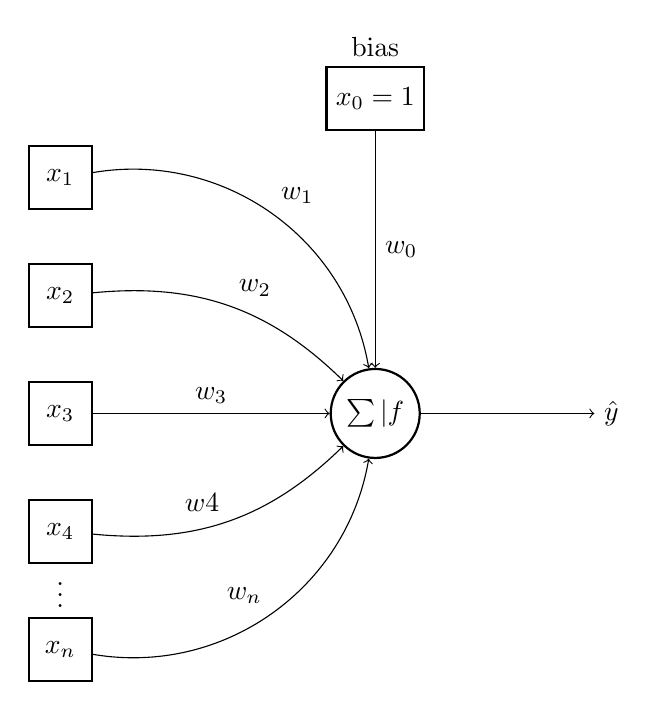
\begin{tikzpicture}
[neuronnode/.style={circle, draw=black, thick, minimum size=10mm},
 inputnode/.style={rectangle, draw=black, thick, minimum size=8mm}]
\node[neuronnode]	(neuron) at (0,0)	{$\sum|f$};
\node[inputnode]	(bias)	 at (0,4) [label=above:bias]	{$x_0=1$};
\node[inputnode]	(input1) at (-4, 3) {$x_1$};
\node[inputnode]	(input2) at (-4, 1.5) {$x_2$};
\node[inputnode]	(input3) at (-4, 0) {$x_3$};
\node[inputnode]	(input4) at (-4, -1.5) {$x_4$};
\node at (-4, -2.2) {$\vdots$};
\node[inputnode]	(inputn) at (-4, -3) {$x_n$};
\node (output) at (3,0) {$\hat{y}$};
\draw[->] (input1) to [bend left=45] node[auto] {$w_1$} (neuron);
\draw[->] (input2) to [bend left=25] node [auto] {$w_2$}(neuron);
\draw[->] (input3)  -- node[auto] {$w_3$} (neuron);
\draw[->] (input4) to [bend right=25] node[auto] {$w4$} (neuron);
\draw[->] (inputn) to [bend right=45] node[auto] {$w_n$} (neuron);
\draw[->] (neuron.east) -- (output);
\draw [->] (bias.south) -- node[auto] {$w_0$} (neuron.north);
\end{tikzpicture}
\end{document}